%
%	Begrifflichkeiten
%

\pagebreak
\section{Data Sources and Research Methods}

\onehalfspacing

\subsection{The blog}

Text

\subsection{Plausible}

\begin{figure}[H]
\centering
\caption {Plausible Summary}
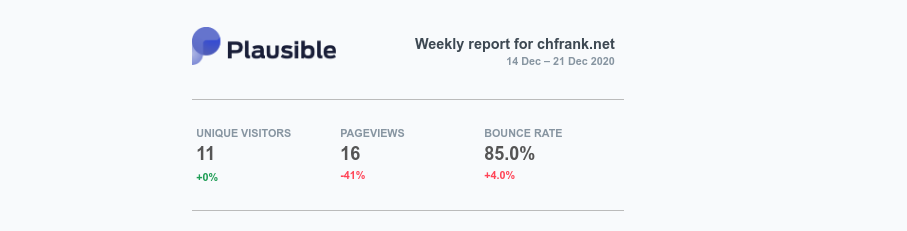
\includegraphics[width=\linewidth]{images/plausible.png}
\label{fig:plausibleSummary}
\end{figure}

In a previous paper, I have covered Kubernetes in more detail\footnote{See \textit{Frank, C. (2020)}: Multi-Cluster Management fuer Containerumgebungen .\cite{previousPaper}}, in this paper I will only cover the necessary basics.

\subsection{Statistical Methods}

Text

\subsection{Sentiment Analysis}

Text

